\section{QoI Model}
\label{sec:qoi_model}

The difference between Quality of Information and the traditional notion of network performance, called Quality of Service (QoS), is an important distinction to be made.  While QoI has some connection to metrics like throughput, delay, jitter, packet loss, etc., its meaning goes beyond objective measurements.  The true value of data in terms of QoI relies on its utility within the context of its use.  A simple example of QoI is relating it to its importance in assisting a user with making or improving the confidence in a decision.  Here, depending on a number of factors, such as timeliness, freshness, completeness, uniqueness, etc., a packet sent across the network may have very different impacts on the receiving end.  For that reason, these various (often contextual) qualities of data are examples of the metrics used to determine the utility or QoI of a piece of data.  To use these metrics in functional ways, applications keep vectors of the chosen attributes for data items.  When a scalar value is required, one can be determined by inputting the vector into a designed QoI function that is weighted to prioritize specific attributes as the end user desires.

%QoI describes collected information in terms of any number of attributes such as accuracy, timeliness, freshness, credibility, completeness, or diversity.  These attributes go beyond standard network metrics like delay, throughput, jitter, and packet loss, which are more akin to the more traditional notion of Quality of Service.  QoI is commonly represented by a vector of the chosen attributes.  With this vector, a scalar value can be obtained by inputting it into a designed QoI function, which can be weighted to prioritize specific attributes if the end user desires.  

%When considering QoI, the utility of each piece of data extracted from a sensor or military tactical network is highly dependent on its context with respect to the network's goals and the other data collected.  
Even though QoI is highly contextual and customizable to a specific network and its goals, our goal here is to show how it can be effectively used in network design.  To that end, we introduce several metrics here that provide real examples of how QoI can be measured quantitatively as described above.  Specifically, we will adopt a notion of \emph{completeness} to use as QoI within this work, showing how it can be defined in the contrasting situations of users having an underlying knowledge of the information available or needing to acquire the scope of available knowledge with some level of confidence. 

We will also identify three example applications and accompanying algorithms that motivate using completeness as an effective network goal.  We note that QoI and its usage in understanding networks is not exclusive to these metrics and applications.  On the contrary, the model used in the scalability analysis of Section \ref{sec:qoi_scalability} can be used with any feasible QoI requirements.

\subsection{Image Selection Algorithms}

As a motivating example, we choose an ad hoc network in which nodes generate photographs that are to be exchanged or collected at one or more data sinks.  This example covers surveillance missions of military tactical networks or social applications for civilians, one example of which could be smartphone users contributing to an image-sharing application. 

The first application in this setting that we introduce is as follows:  Given the set of all photographs available in the network, we would like to return the set of $k$ that exhibits the most diversity, ideally providing a user with a good sampling of images available in the network.  This result is known as the {\bf Spanner} of the set of known photographs.  Such a result would be useful in a surveillance mission or in a social setting in which users would like a quick idea of the current state of a large area or event.  

A similar approach to achieving this goal of discovering a complete view of the environment the network is sensing is to use the second algorithm we consider, which we simply call {\bf Clustering}.  Here, all images are separated into $k$ clusters based on their pairwise distances using any version of a k-means clustering algorithm.  Then, the most central photograph from each cluster is returned.  Here, assuming that the photographs of the same settings or objects of interest exhibit similar characteristics, {\bf Clustering} should provide a complete view of the environment in which the network is operating.

The final application we introduce occurs when one already has an image of a particular area or object of interest and would like to obtain similar images to get a more complete view of that specific scene or object.  For example, if a user observes a picture of an unknown suspicious person entering a building, but the person is not identifiable from that image, it would be useful to collect more images that are similar to that one with the possibility that another picture of the building from another source may have a better view of the person in question that can be used for identification or more context.  In a social situation, a user may want more images of a particular event of interest like a parade, a concert, or a sporting event.  Called {\bf Top-K}, the algorithm used for this application will choose the $k$ images with the most similarity, or \emph{smallest distance}, from the given image.  

We note that while metadata associated with photographs may be useful in obtaining similar goals, content-based retrieval can sometimes be more effective, or at the very least can be used in addition to metadata to improve accomplishing the set goals.  For instance, all of the images could be tagged with location and time stamps allowing an application to filter for desired values to get matching or spanning images sets.  Even a location and time stamp will not account for the direction that the photographer is facing or objects in between the camera and a desired object or person of interest.  Content-based processing of these images, though, can be applied to the set of photographs existing after any location or time filtering to improve the Spanner, Clustering, and Top-K algorithm results on these image pools.  

\subsection{Image Similarity}

To implement these algorithms, we again use the same choices for measuring the similarity of two images as was shown to be effective in \cite{mediascope}.  This similarity is based on qualities inherent to a photograph like lightness, contrast, and color.  While many techniques have been studied to compare photographs using these qualities, we choose an image-processing technique called Color and Edge Directivity Descriptor (CEDD) \cite{2008cedd}.  With CEDD, each image is described by a vector of 144 different features describing color and spatial color distribution.  

We achieve a scalar representation of similarity between two images by calculating the \emph{Tanimoto Similarity}, $T_s$, between their CEDD feature vectors, another practice commonly used in the image processing community \cite{tanimoto}. The Taminoto similarity metric is defined as follows: Given two images with feature vectors $\mathbf{a}$ and $\mathbf{b}$,
  \begin{equation}
  T_s(\mathbf{a,b})=\frac{\mathbf{a.b}}{\mathbf{a.a+b.b-a.b}},
  \end{equation}
where $\mathbf{a.b}$ is the inner product of two vectors. Proper normalization keeps this metric in the $[0,1]$ range. Naturally, to describe the dissimilarity, or distance, of two photographs, then, we simply use $T_d = 1 - T_s$.

\subsection{Measuring QoI}

As already discussed, \emph{Quality of Information} is a very contextual term, so defining metrics to provide objective measurements of it is a challenge within itself.  Here, we provide methods for measuring completeness of a collected set of images with respect to the pool of all available images.  First, we will explain how the similarity and dissimilarity for varying numbers of collected photographs, $k$, can be used to describe the QoI of each algorithm.  Then, we will also show the resulting QoI with respect to specific scenarios with known ground truths to give real-world examples of how QoI differs dramatically from QoS.

\subsubsection{Unknown Information Space}
For the Spanner algorithm, we employ a greedy algorithm similar to that in \cite{mediascope} to simplify implementation and to define a \emph{Sum Dissimilarity} metric.  Here, the algorithm first chooses the two images with the greatest distance between them from all available images.  Then, each successive image is chosen to be the one with the greatest minimum distance between it and all images already chosen, until $k$ images are selected.  This minimum distance between the image being selected and the images in the collected set is the value added to the running cumulative QoI metric of \emph{Sum Dissimilarity}.  Since the Spanner algorithm's goal is to provide images at the edges of the available feature space, the Sum Dissimilarity represents a measure of its effectiveness.  Here, a higher level of dissimilarity is providing a more complete view of the feature space itself.

%To cluster the images, a $k$-means clustering algorithm is used with the image closest to the centroid of each of the $k$ clusters being selected.  

Conversely, the Top-k algorithm's goal is to provide images with features that are similar to the target image.  Therefore, the Tanimoto Similarity of each successive image gives its effectiveness in providing a more complete view of the object or scene of interest.  Naturally, then, the \emph{Sum Similarity} of each successive image returned by the Top-k algorithm is a measure of the completeness being achieved.

Figures \ref{fig:topkSumSim} and \ref{fig:spanSumDissim} show the average sum dissimilarity and similarity of images returned by the Spanner and Top-k algorithms, respectively, run on a set of images collected over the Penn State campus.  These figures exhibit the diminishing returns of using similarity and dissimilarity metrics.  This effect is important also because it visually shows how Quality of Information differs from throughput.  As seen in these graphs, transmission of successive images is not linear in terms of gained completeness.  Inversely, this relationship shows that obtaining a certain value of QoI or completeness may require a different number of images depending on the set available and their similarities.  Specifically, we can denote the number of images required to achieve a level of completeness, $S$, as $N(S)$.  This relationship will be useful later in determining feasible scalability.

%Spanner Sum Dissimilarity
\begin{figure} 
\begin{centering}
    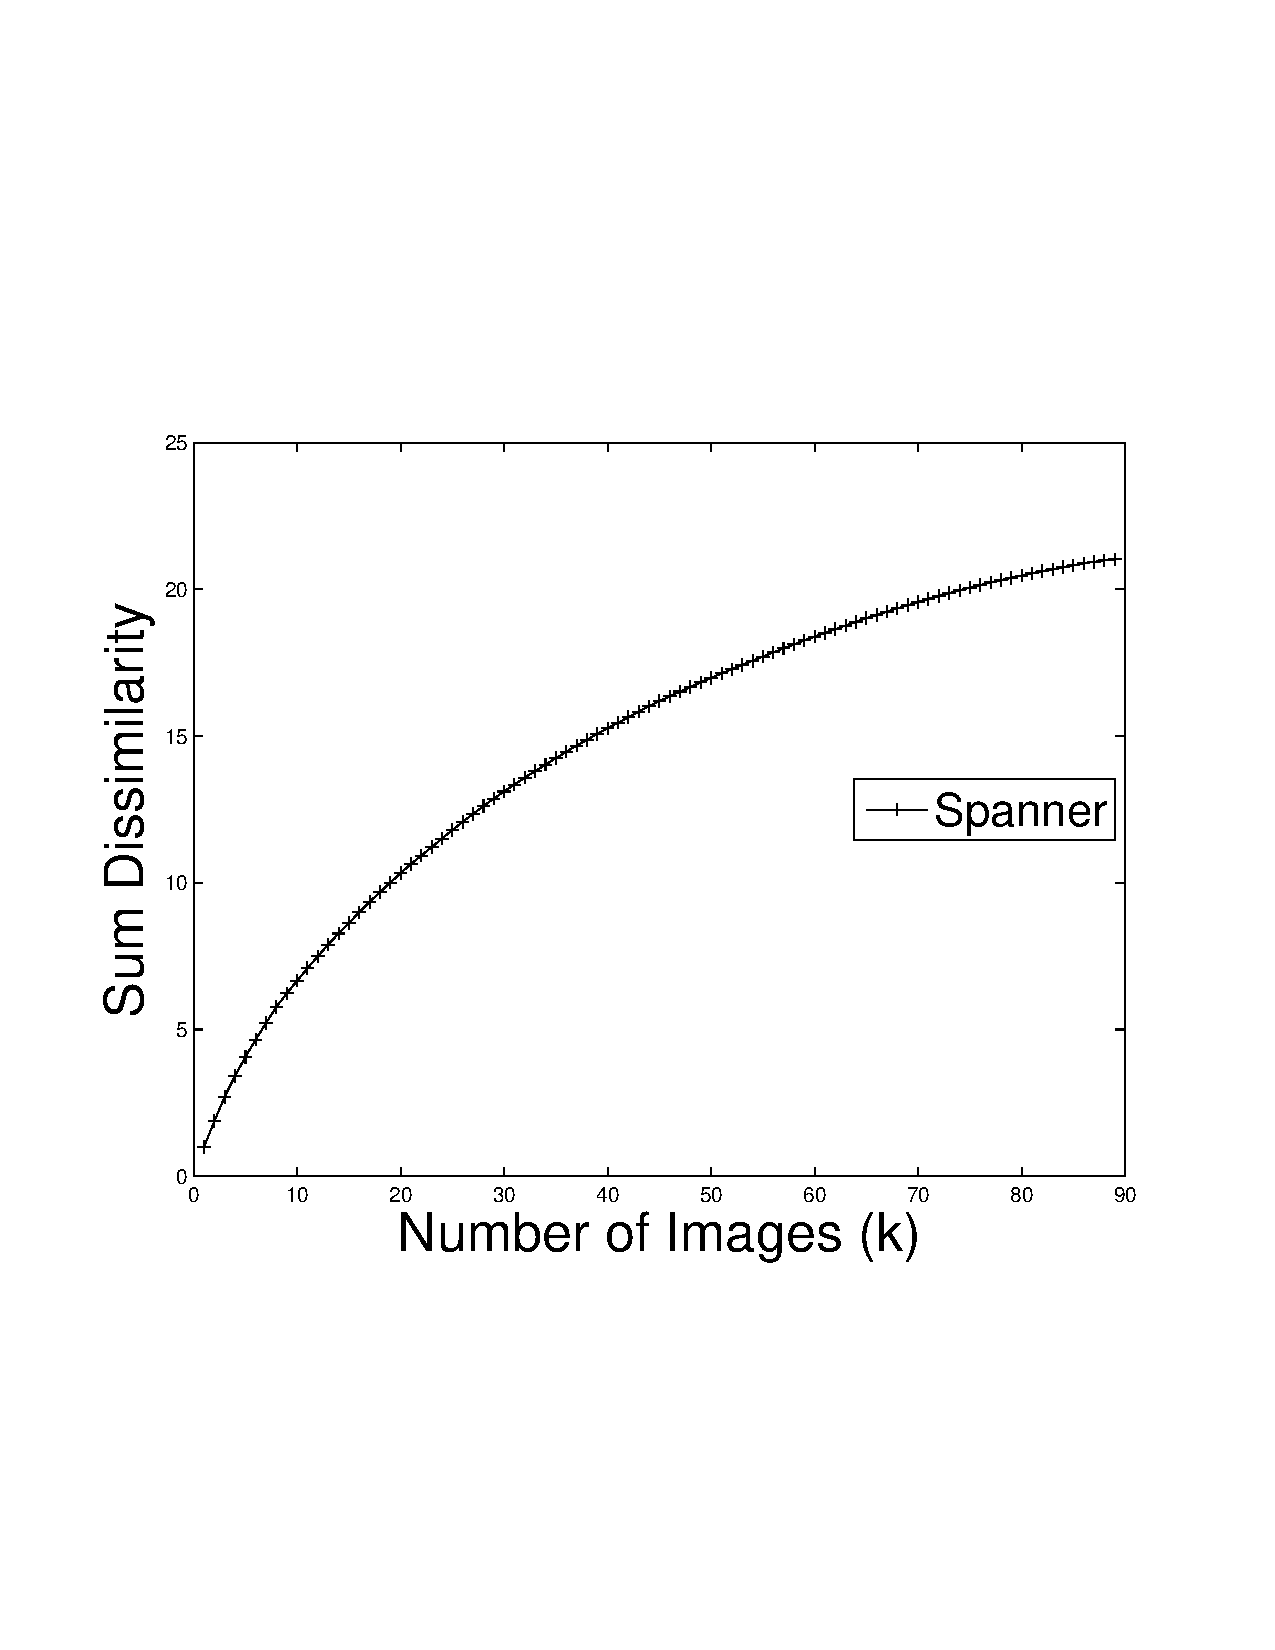
\includegraphics[trim = 0mm 70mm 0mm 70mm, scale=0.40]{figures/spanner/spannerCumulativeDist.pdf}
    \caption{Sum Dissimilarity for Spanners of Varying $k$}
    \label{fig:spanSumDissim}
\end{centering}
\end{figure}

%%Cluster Sum Dissimilarity
%\begin{figure} 
%\begin{centering}
%    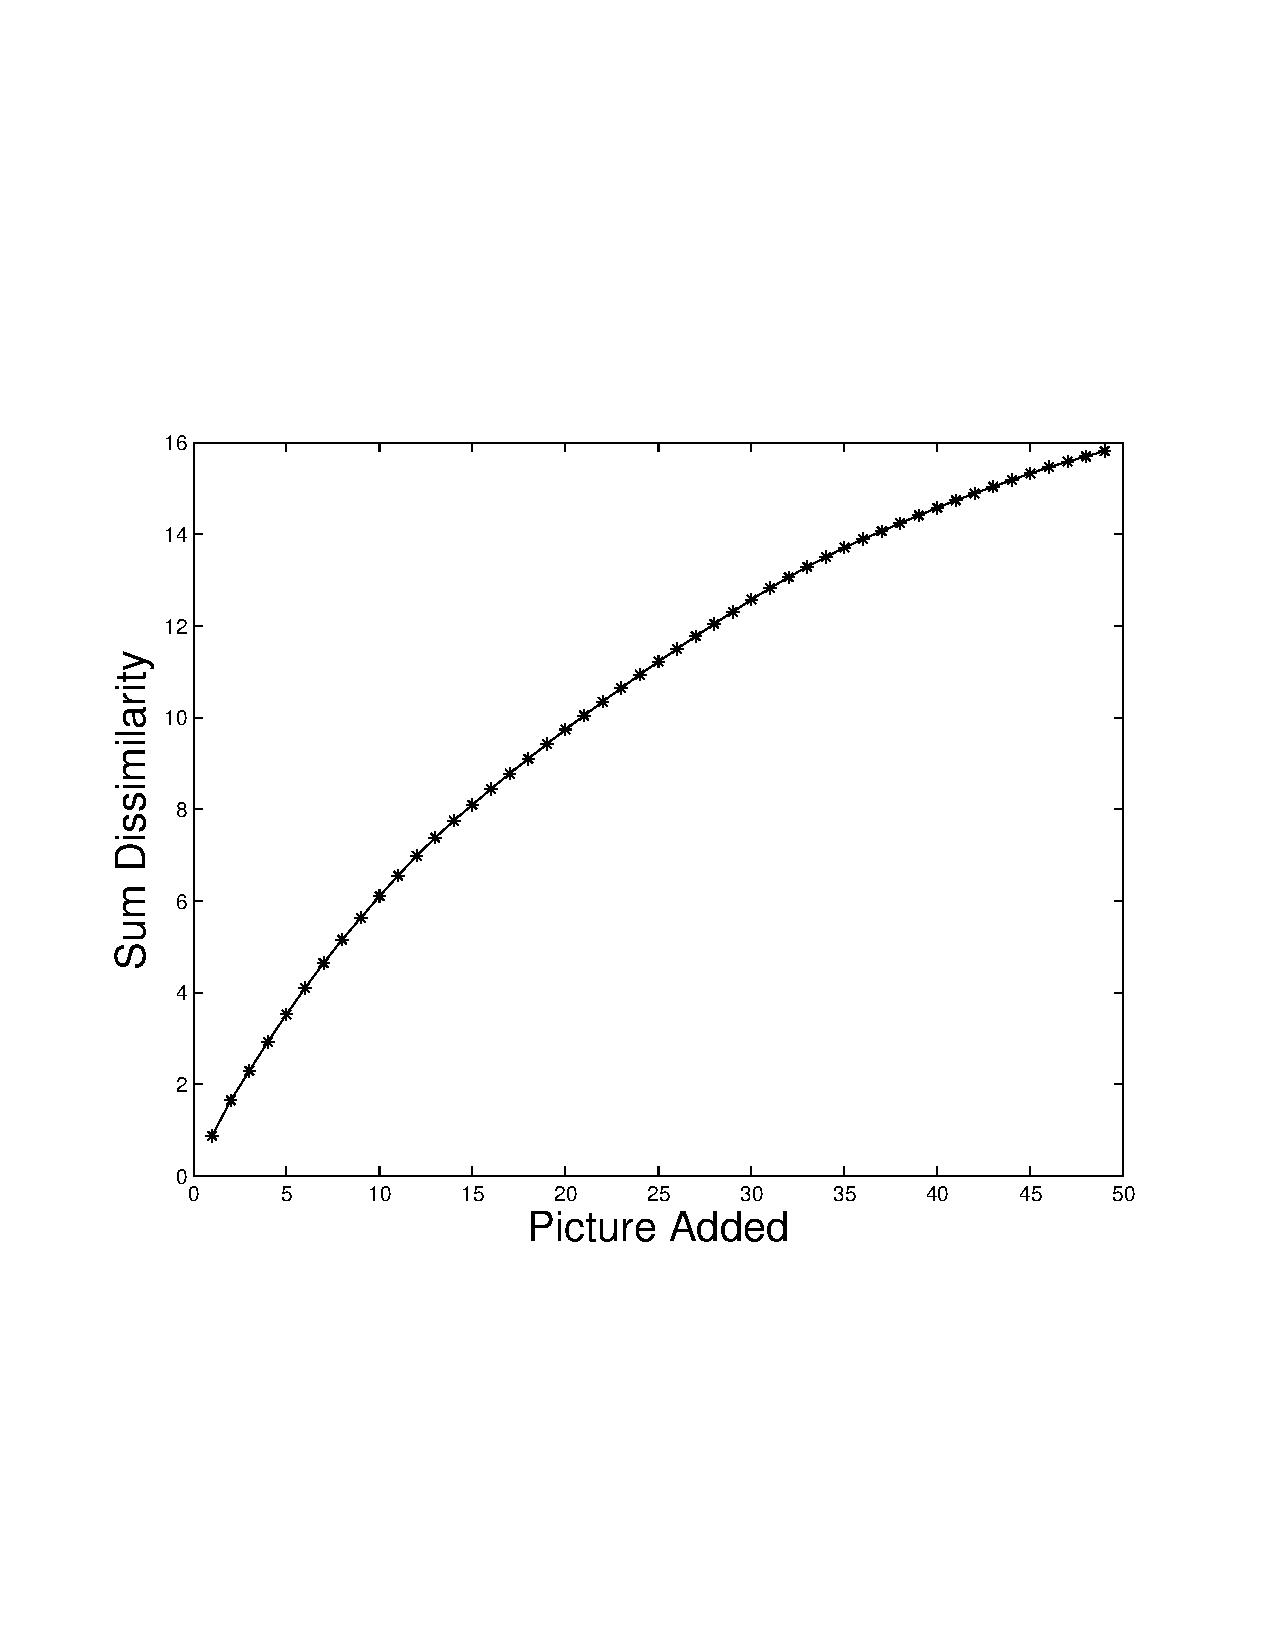
\includegraphics[trim = 0mm 70mm 0mm 70mm, scale=0.40]{figures/cluster/sum_dissimilarity_like_spanner.pdf}
%    \caption{Sum Dissimilarity for Varying Number of Clusters, $k$}
%    \label{fig:clusterSumDissim}
%\end{centering}
%\end{figure}

%Top-k Sum Similarity
\begin{figure} 
\begin{centering}
    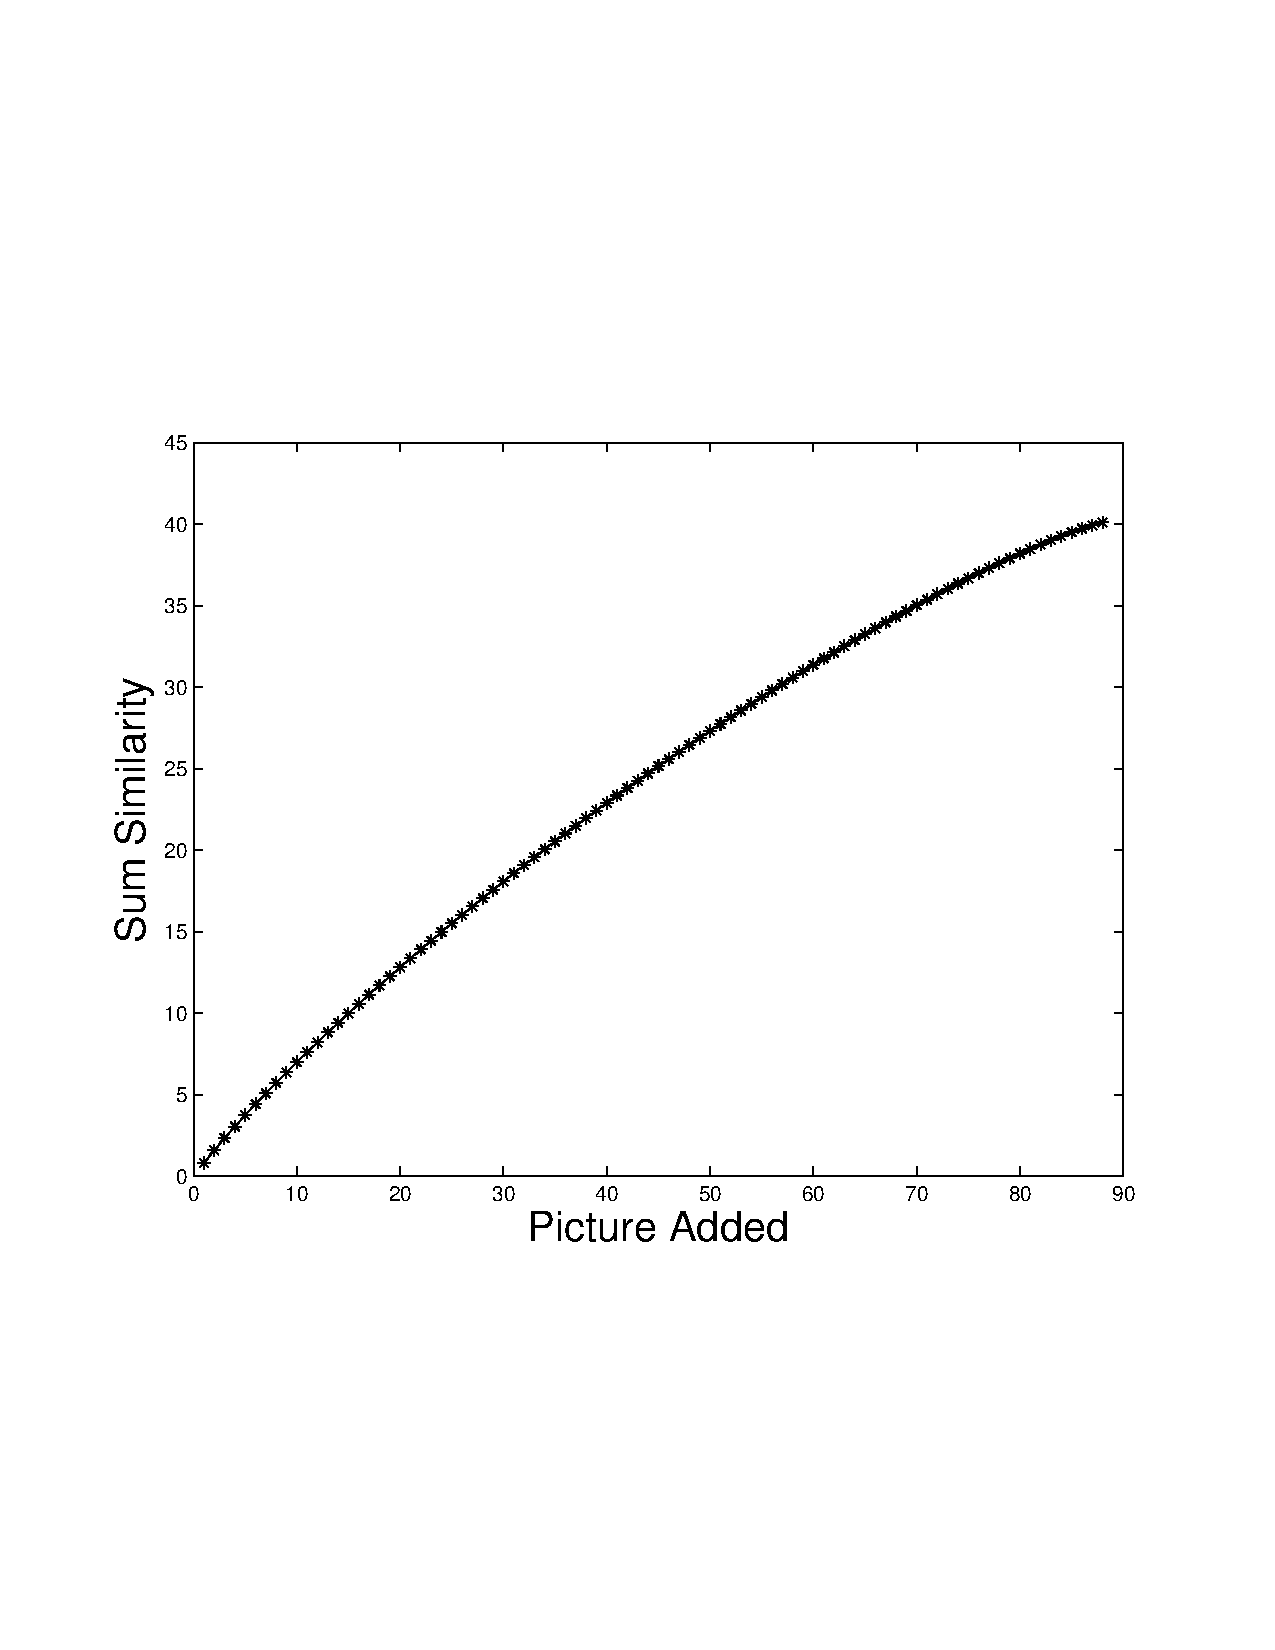
\includegraphics[trim = 0mm 70mm 0mm 70mm, scale=0.40]{figures/topk/topk_sum_sim.pdf}
    \caption{Sum Similartiy for Top-K Results of Varying $k$}
    \label{fig:topkSumSim}
\end{centering}
\end{figure}

\subsubsection{Known Information Space}
For our approach to measuring QoI, we can use a model in which each image belongs to one of $n$ sets, $Q_n$, which can each represent a particular setting of interest.  Naturally, then, when executing a Top-K query, the goal is for the algorithm to return images from the same set as the target image.  In the case of a spanner query, the goal is to return images from different sets.  

Using these two naturally occurring goals, we can measure the effectiveness of the algorithms, providing QoI values.  For Top-K, the QoI value is the number of photographs returned that are in the same set as the target image.  For the spanner algorithm, the QoI value can either be the number of sets covered by at least one of the returned images, or it can be the likelihood that all $n$ sets will be covered by the returned images, as long as $k \geq n$.

To provide example values of these QoI metrics, experiments were run on photographs taken at $5$ different settings around the Penn State campus.  Each of the settings is of a pictorially different setting, e.g. a particular building, a downtown street, or a lawn setting, and over $20$ images of each was taken.  Then, for individual trials, sets of $Q_n$ with $10$ images in each set were randomly selected from this group of photographs and the Top-K and spanner algorithms were run over these $50$ images with the target image being randomly selected in the case of Top-K.

Figures \ref{fig:topkAvgNumSameSet}-\ref{fig:spannerAvgNumSetsCov} show the average results of 1000 trials.  In Figure \ref{fig:topkAvgNumSameSet}, it is evident that a value of only $k \approx 10$ is needed to collect $5$ images matching the target content, while collecting an additional $2$ from the same usually requires collecting over twice that number of pictures.  

This diminishing return is also evident in the spanner algorithm results.  Figure \ref{fig:spannerAvgNumSetsCov} shows the number of sets represented by the algorithm output for increasing $k$.  Here, if the goal is to achieve at least one image from each of the different settings as might be in a surveillance application, the spanner achieves it on average at $k \approx 17$.  The same trend is evident in Figure \ref{fig:spannerAvgPercAllSetsCov} where the probability of covering all sets is plotted against $k$.  Using this metric, the application can use the probability of achieving full coverage as the QoI metric.  From this example application, if collecting at least one image from each set with $90\%$ probability of success is acceptable, then only $k=13$ images are necessary.

%% Spanner Percentage All Sets Covered
%\begin{figure} 
%\begin{centering}
%    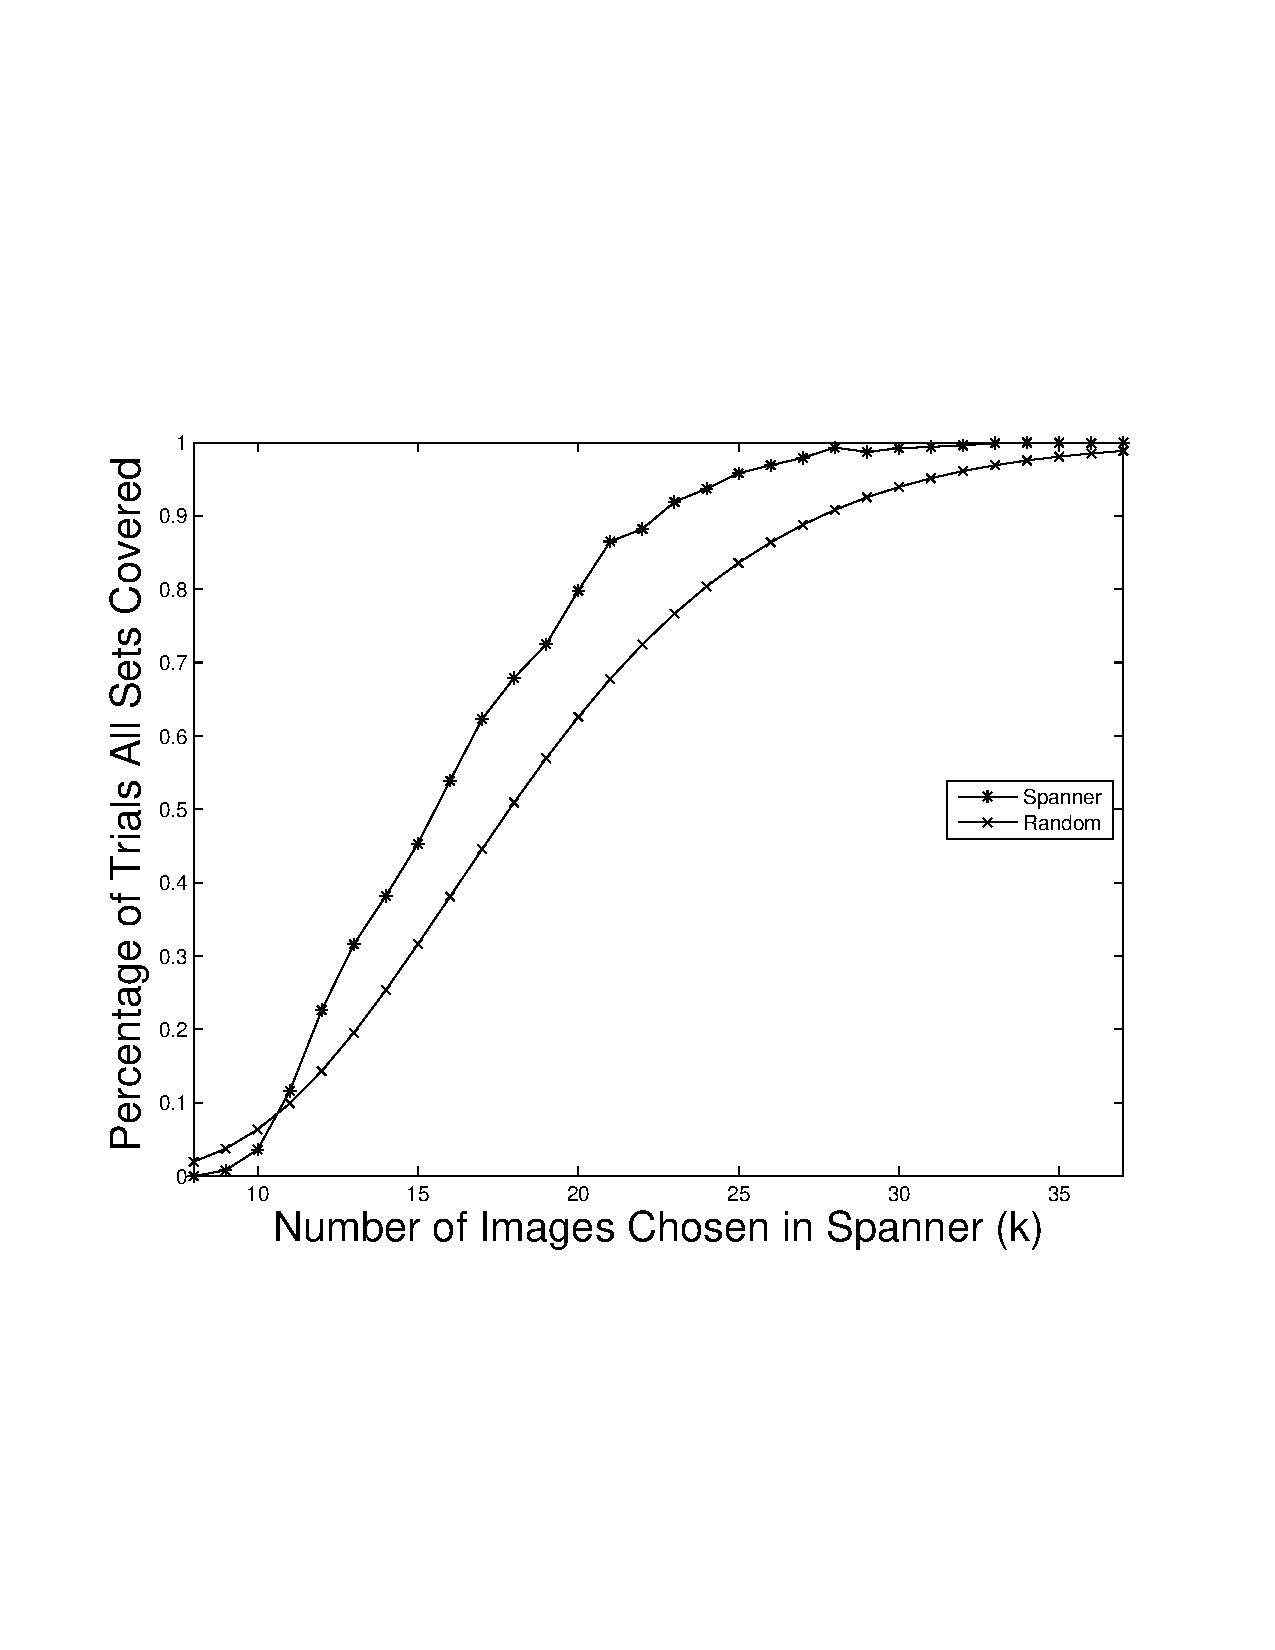
\includegraphics[trim = 0mm 70mm 0mm 70mm, scale=0.40]{figures/spanner/perc_all_sets_covered.pdf}
%    \caption{Average Percentage All Sets Covered by Returned Images}
%    \label{fig:spannerAvgPercAllSetsCov}
%\end{centering}
%\end{figure}

% Cluster Percentage All Sets Covered
\begin{figure} 
\begin{centering}
    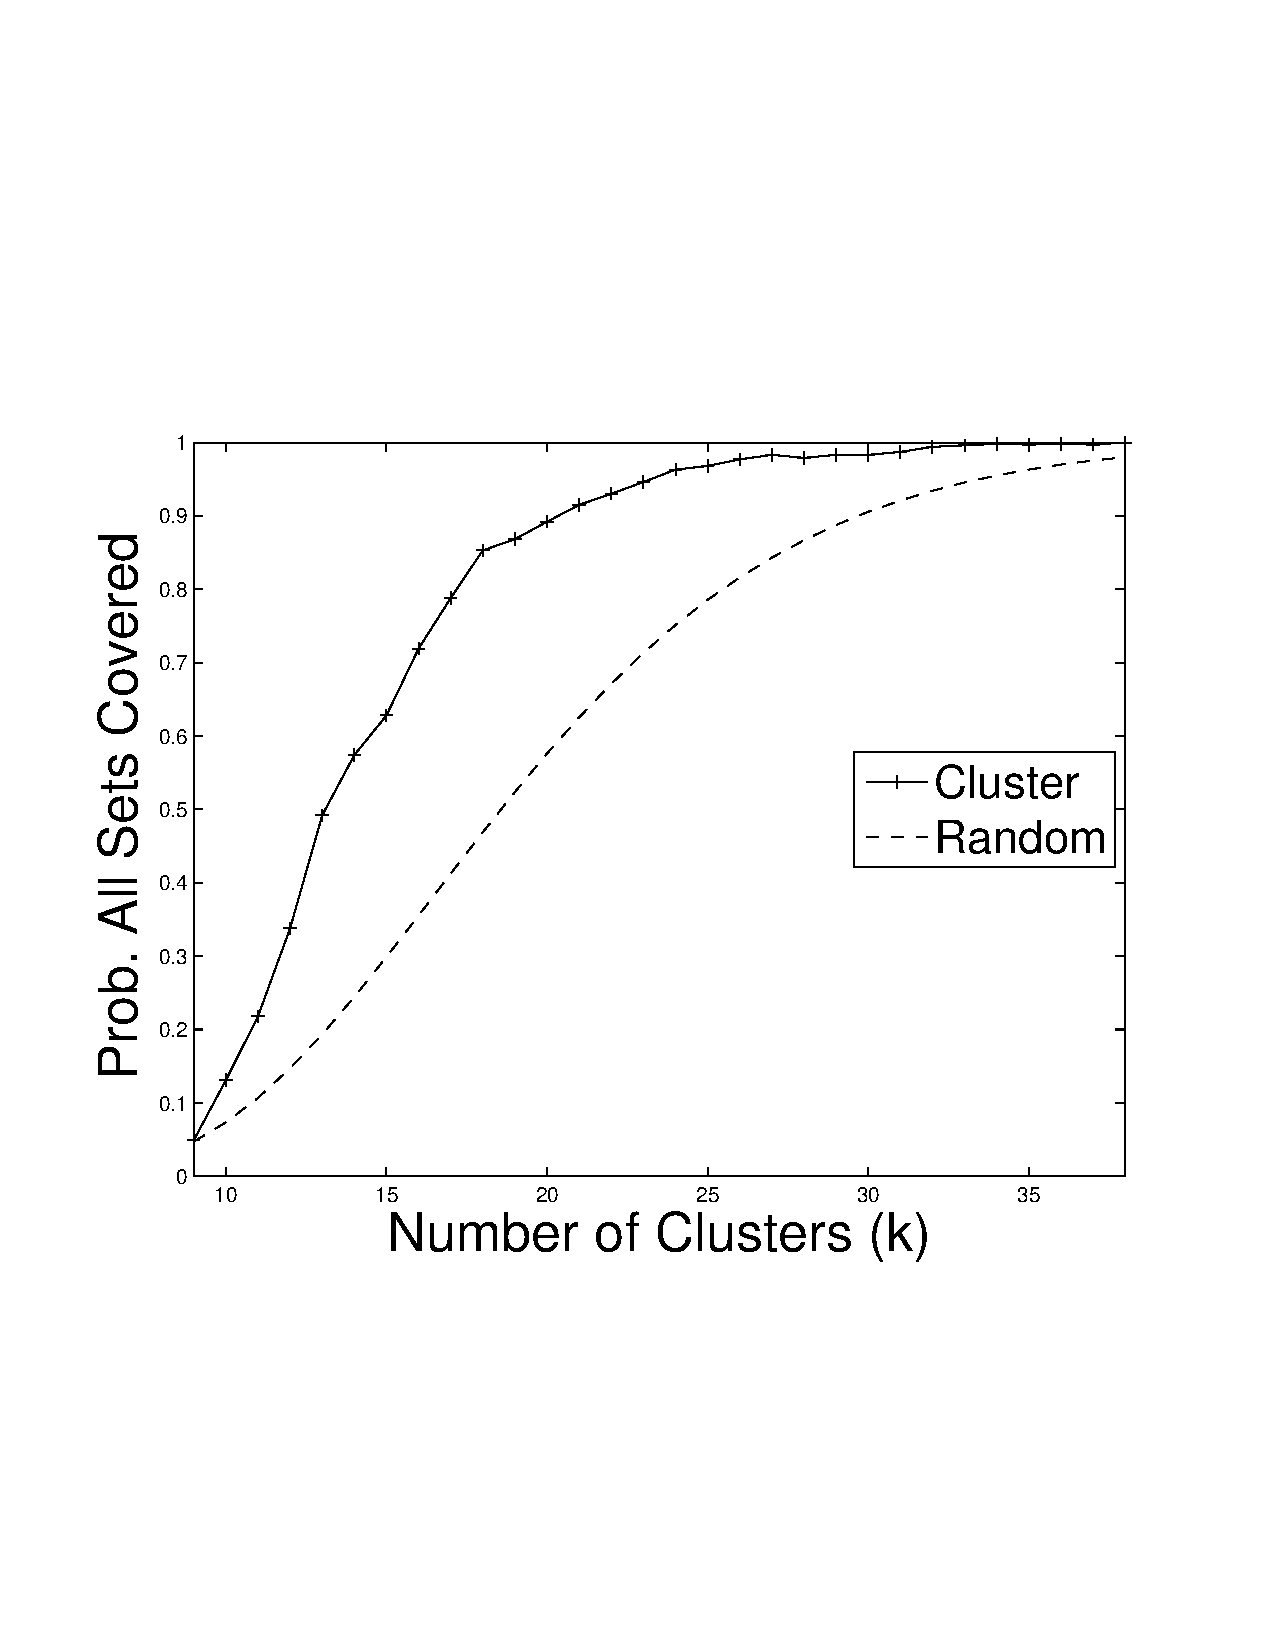
\includegraphics[trim = 0mm 70mm 0mm 70mm, scale=0.40]{figures/cluster/perc_all_sets_covered_vary_k.pdf}
    \caption{Average Number of Sets Covered by Returned Images}
    \label{fig:spannerAvgNumSetsCov}
\end{centering}
\end{figure}

% Top-K Average Number from Same Set Returned
\begin{figure} 
\begin{centering}
    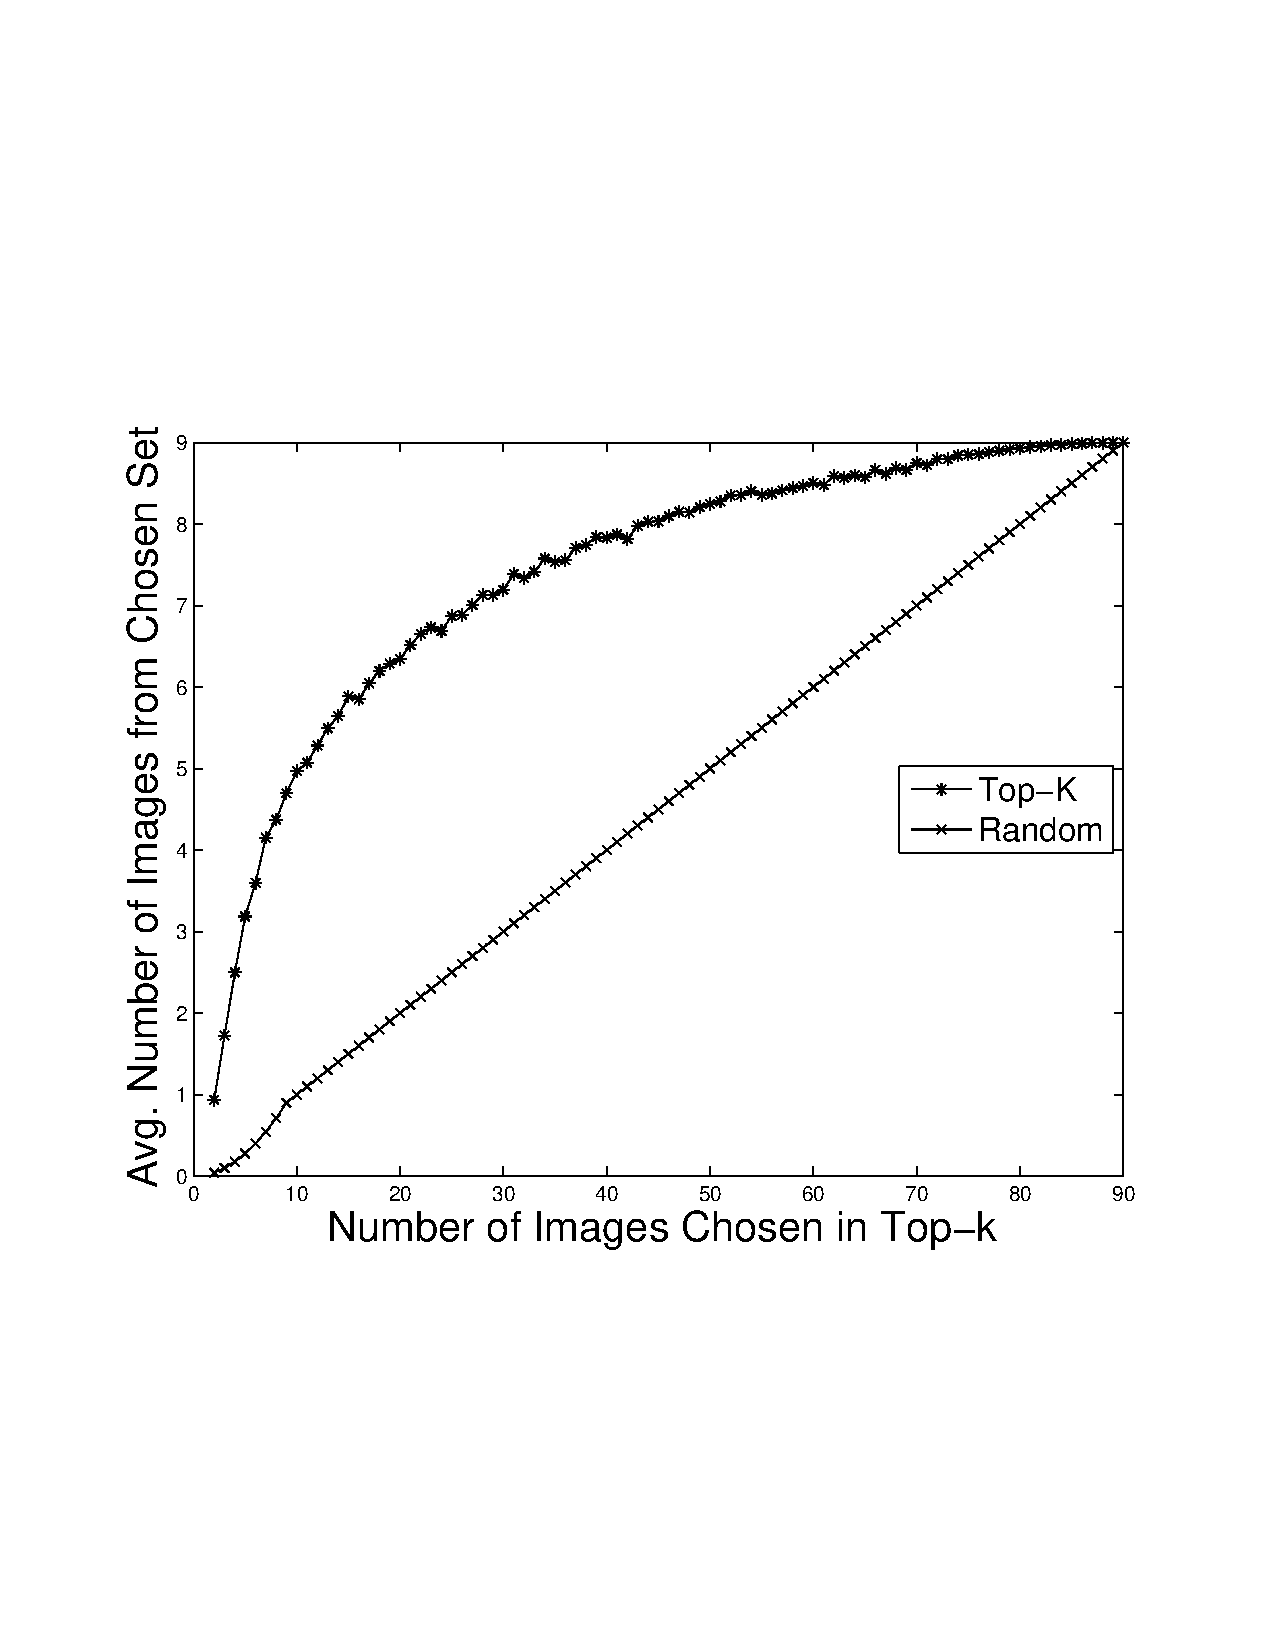
\includegraphics[trim = 0mm 70mm 0mm 70mm, scale=0.40]{figures/topk/avg_num_matching.pdf}
    \caption{Average Number of Images Selected from Same Set as Target Image}
    \label{fig:topkAvgNumSameSet}
\end{centering}
\end{figure}

Comparing Figures \ref{fig:topkSumSim}-\ref{fig:spanSumDissim} with Figures \ref{fig:topkAvgNumSameSet}-\ref{fig:spannerAvgPercAllSetsCov}, we observe that completeness and diversity provide a sound indication of the number of sets covered for different numbers of images collected, encouraging our choice of focusing them as QoI attributes.


%As for how we were planning to relate a notion of QoI which is increasing with more images;
%The Top_K query seems readily expandable for different K-you give a target image and as you collect more images you add more "similarity metrics"(which reduces with distances), but the spanner had some issues:
%If normalized among all distances, the average distance among elements reduces with more elements.
%On the other hand, if we simply add pairwise distances, it overcounts too many combinations (n choose 2)
%So, the latest possibility I had in mind was to consider an additive metric such that each introduced picture brings increases the metric proportion to either the avg distance to existing elements, or minimum/maximum of all distances to the existing elements. 
%Given the definition of "spanner", which is "Spanner maximizes the minimum dissimilarity between all pairs", what  I had in mind was perhaps to consider an additive metric such that each introduced picture increases the metric proportion to the minimum of all distances to the existing elements. Or, since the whole set of selected pictures might change with different 
%K, probably the best metric is:
%
%For a spanner of K pictures: Total "quality/diversity metric" = \sum_{i=1 to K} min_{j in K-i} (distance_i, j)
%
%that is, we run the spanner, find K pictures. For each picture we have a minimum dissimilartity/distance to rest of the pictures. Than, we add these minimum dissimilarities over all pictures. 
%I think the case where the extra metric added is in proportion to the average distances should decrease for each new added picture, so we should have a increasing concave type function.

%the graph is generated as follows: 
%given a timeliness T and dissimilarity(D)/similarity(S) requirement, we find how many nodes the network can scale up to, say N, by the scalability analysis formulas.
%Then we look at how many images are required for attaining D/S, say K(this comes from the CEDD based MATLAB analysis). With the assumption that each node has one image, this essentially implies a lower bound on the required network size in terms of number of nodes to attain D/S.
%If N<K, the network cant actually scale large enough to provide the similarity/dissimilarity, so it is not "scalably feasible".
%so this graph is obtained as follows; for each T, identify the largest D/S such that N>=K still holds.